\documentclass[main]{subfiles}

\begin{document}

\section{Eksperimentel Opstilling}
Delforsøg 1 og 2 har identisk opstilling på følgende punkter: En laser kilde pkt. 1 på \cref{fig:opstilling1} og \cref{fig:opstilling2} udsender en laser stråle på $\lambda \approx  \SI{900}{\nano\m} $. Herefter rammer laseren en linse, pkt. 2, der har til formål at danne en kollimeret laser stråle, hvorefter strålens føres over i AOM'en pkt. 5, via. 2 spejle pkt 3. og en linse pkt. 4, der fokusere laser strålen i AOM'ens indgang.

\subsection{Delforsøg 1}
I dette forsøg, er AOM'en forbundet til en frekvensgenerator og en forstærker på hhv. pkt. 8 og 7 på \cref{fig:opstilling1}. Herefter bliver laser strålen diffraktions ordner, som rammer en skærm pkt. 6.
\begin{figure}[H]
    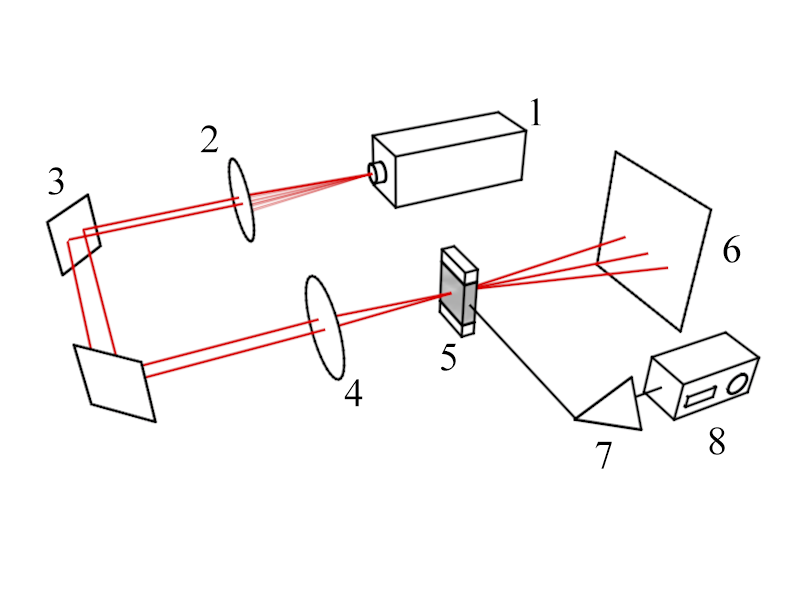
\includegraphics[width=\linewidth]{tegninger/tegning1.png}
    \caption{Opstilling til delforsøg 1.}
    \label{fig:opstilling1}
\end{figure}

\subsubsection{Dataopsamling}\label{dataopsamling1}
Først sørges for at laseren rammer AOM'ens indgang. Herefter finjusteres AOM'ens position og vinkel, således at $1^{st}$ ordens diffraktionsstrålens intensitet maximeres, ved at bruge en powermeter. Nu måles afstanden mellem $0^{th}$ ordens og $1^{st}$ ordens strålernes position på skærmen (pkt. 6 \cref{fig:opstilling1}), som funktion af frekvensen som udsendes af frekvensgeneratoren.
\\ Sidst måles intensiteten af $1^{st}$ ordens strålen som funktion af frekvensgeneratorens effekt-output, ved hjælp af en powermeter.


\subsection{Delforsøg 2}\label{dataopsamling2}
Til forskel fra delforsøg 1, placeres en switch pkt. 9, i mellem frekvens generatoren og forstærkeren på \cref{fig:opstilling2}. Switchen er også tilkoblet et oscilloskop med indbygget frekvensgenerator. Dette tilkobles ved en $\SI{50}{\ohm}$ tilkobling for at sikre at en måling kan detekteres da vi gerne vil simulere at AOM'en er tilkoblet.  Skærmen pkt 6. Er brugt til at afskærme den ene stråle, hvorefter den anden stråle opsamles på en fotodetektor i pkt. 10. I praksis, er føleren på fotodetekteren meget lille, så der anvendes en linse til at fokusere beamen på detekteren. Ud over det, anvendes der også et oscilloscop til at logge spændingen.

\begin{figure}[H]
    \centering
    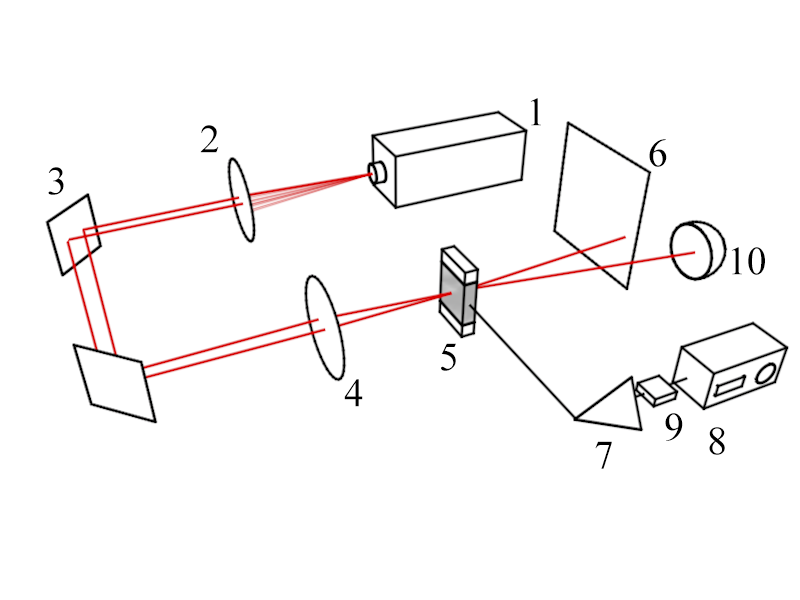
\includegraphics[width=\linewidth]{tegninger/tegning2.png}
    \caption{Opstilling til delforsøg 2.}
    \label{fig:opstilling2}
\end{figure}

\subsubsection{Dataopsamling}
I oscilloskopet er der indbygget en frekvensgenerator som her sender et signal over til switch'en som da skifter hurtigt mellem on/off. Først holdes AOM'en udenfor dette kredsløb så vi kan notere hvor hurtigt signalet kan skifte, hvilket gøres ved at skrue op for frekvensen og se at switchen følger med. Når dette er udført er vi sikre på at vi kan sende et signal som er hurtigt nok til at skifte signalet til AOM'en meget hurtigt, hvorfor vi slutter AOM'en til kredsløbet igen.
\\
Nu ønskes det at bestemme waist. Først vil vi gerne sikre os at laserstrålen er gaussisk. Dette gøres ved at måle intensiteten som funktion af hvor meget af strålen vi blokerer. I praksis gøres dette ved at tage et barberblad på en millimeter-skrue og køre den ind foran strålen i fokallængden fra linsen. Imens dette gøres måles intensiteten af laserstrålen med en powermeter. Data tjekkes til at tilhøre en gaussisk stråle. Da dette gælder kan man finde waist, ved at tage forskellen i længden mellem de to punkter hvor laserstrålen blokeres, således at  intensiteten formindskes med 16 og 84 \%.
\\ Nu sættes AOM'en ind i det punkt hvori vi målte waist. Da vi havde sat switchen op kan vi nu tænde og slukke for lydbølgen i AOM'en meget hurtigt hvorfor vi kan måle hvor langt tid det tager for lydbølgen at bevæge sig hen over laserstrålens bredde, idet at vi har sat en fotodetektor op i $1^{st}$ ordens laserstrålen (pkt. 10 \cref{fig:opstilling2}). Dette gentages i forskellige bredder af laserstrålen, altså ved at sætte linser med forskellige fokallængder ind. I praksis anvende osciolscopets cursor mode, på et datasæt hvor falltime noteres, som vist i  \cref{fig:osciolo}.
\begin{figure}[H]
    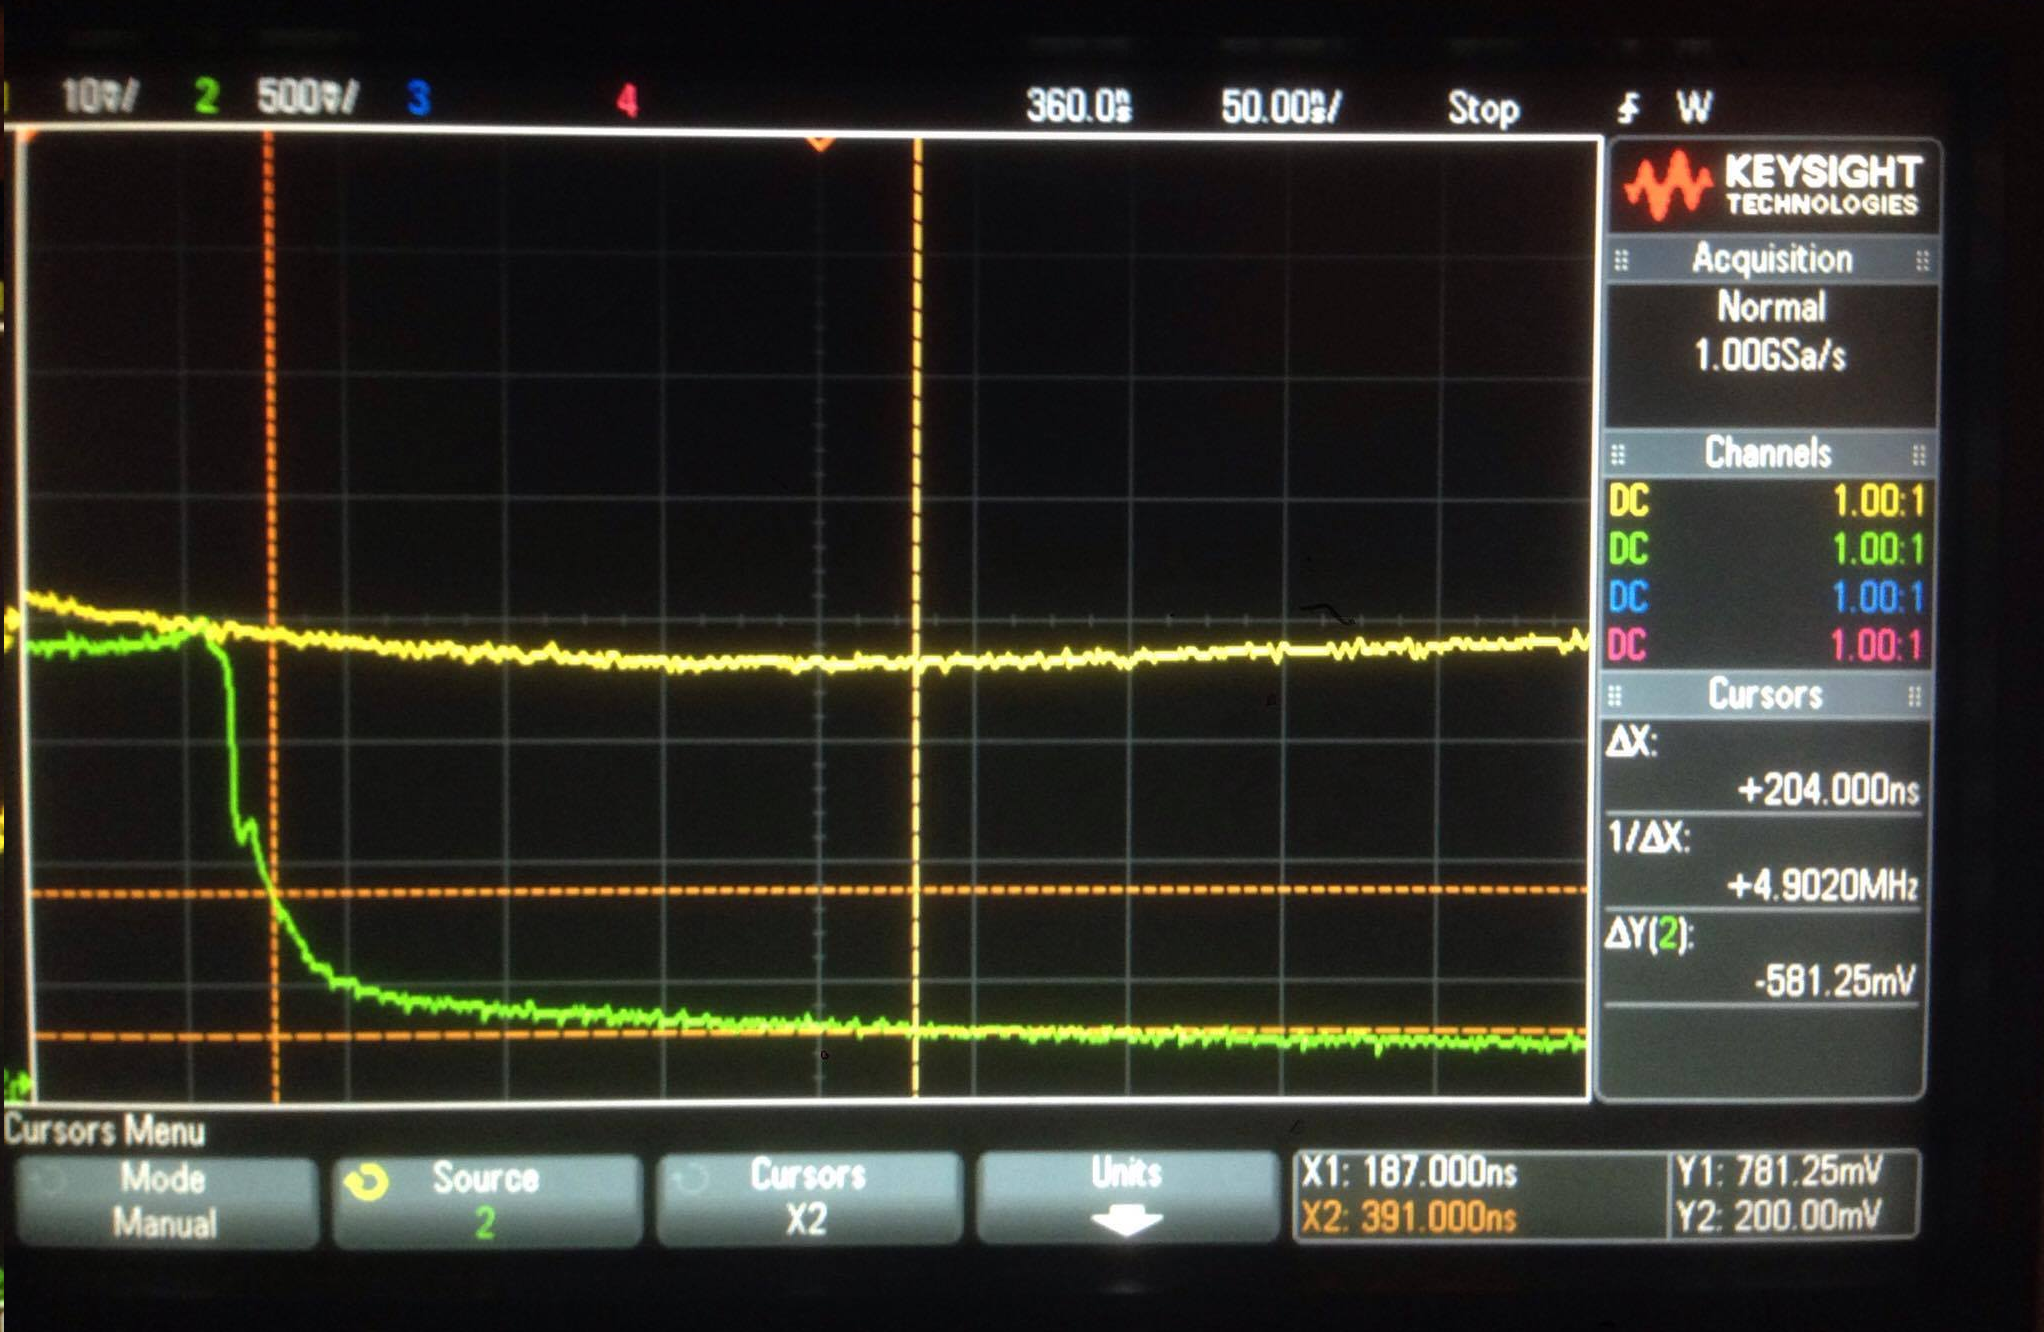
\includegraphics[width=\linewidth]{tegninger/osciolo.png}
    \caption{}
    \label{fig:osciolo}
\end{figure}

\end{document}
